\documentclass[12pt,a4paper,danish,oneside,openany]{memoir} 
% Skabelon af DTU's LaTeX support gruppe, v20090423

\usepackage[utf8]{inputenc} 
%\usepackage{usecases}
\usepackage{vhistory}
\usepackage[danish]{babel} % danske overskrifter
\usepackage[T1]{fontenc}   % fonte (output)
\usepackage{lmodern}       % vektor fonte
\usepackage{graphicx}      % indsættelse af billeder
\graphicspath{ {./Figurer/} }
\usepackage{pdfpages}      % pdf som forside evt
\usepackage{morefloats}    % flere floats til tabeller
\usepackage{array}         % udvidet tabel 
\usepackage{listings}      % kode
% \usepackage{palatino}      % lækker font
% \linespread{1.3}           % kræver lidt mere line spacing
\usepackage{rotating}
\usepackage{tikz}

\addto\captionsdanish{
  \renewcommand{\contentsname}%
    {Indholdsfortegnelse}     %
} % Så bruger vi bare 'Indholdsfortegnelse' i stedet for 'Indhold'

\usepackage{underscore}
\usepackage{a4wide}
\usepackage{mathtools} % matematik - underst¿tter muligheden for at bruge \eqref{}

\usepackage[plainpages=false,pdfpagelabels,pageanchor=false]{hyperref} % aktive links

\usepackage{memhfixc}  % rettelser til hyperref

\usepackage{tipa}
\pretolerance=2500     % højt tal, mindre orddeling og mere space mellem ord.
% 3000 er okey, 1000 er for lidt, 5000 i overkanten, 8000 er for meget..

\usepackage[font=small,labelfont=bf,labelsep=endash]{caption}
 
\pagestyle{headings}

\makechapterstyle{mortenovi}{%
\setlength{\beforechapskip}{0cm}%længde fra top af side til kapitel-overskrifter
\setlength{\afterchapskip}{1cm}%længde fra kapiteltekst til body-tekst
\setlength{\midchapskip}{2cm}%længe mellem kapitelnummer og kapiteltekst
\renewcommand\chapnamefont{\normalfont\Large\scshape\raggedleft}
\renewcommand\chaptitlefont{\normalfont\Huge\bfseries\sffamily}
\renewcommand\chapternamenum{}%default "kapitel"
\renewcommand\printchapternum{%
    \makebox[0pt][l]{%
    \hspace{0.4em}
    \resizebox{!}{4ex}{\chapnamefont\bfseries\sffamily\thechapter}}
    }%"kapitel. x"-linjen og dens boxe og bredder - prøv at sætte xyz ind først på de tre linjer respektivt.
\renewcommand\afterchapternum{\par\hspace{1.5cm}\hrule\vspace{0.5cm}}
\renewcommand\afterchaptertitle{\vskip\onelineskip \hrule\vskip\afterchapskip
}}
\chapterstyle{mortenovi}

\maxtocdepth{subsection} %Only parts, chapters and sections in the table of contents
\settocdepth{subsection}

% \includeonly{forord,testing} % Kompiler kun de kapitler du arbejder med.

\topmargin = 0pt
\usepackage[textwidth = 155mm]{geometry}
\usepackage{tabularx}
\usepackage{booktabs} % http://ctan.org/pkg/booktabs 
\newcommand{\tabitem}{~~\llap{\textbullet}~~}

\begin{document}

\part*{System Design Document}

\begin{versionhistory}
  \vhEntry{1.0}{21.10.14}{anud|ntho|sjri}{Revision}
\end{versionhistory}

\chapter*{Introduction}

\section*{Design goals}

\paragraph{Usability: } The Calendar system should be designed with the goal in mind that it should be fairly easy to use by the Client. 

\paragraph{Response time: } The Calendar system should be quite responsive to user input, and commonly make actions in a matter of milliseconds. 

\paragraph{Extensibility: } The Calendar system should support the opportunity to extend the program and make it interact with different calendar programs such as Google Calendar, Exchange and iCal. 

%\section*{Overview}


\chapter*{Proposed system}

\section*{Overview}

subsection*{Architectural style}
\newline
 We decided to use the MVC pattern as the basic architectural style for the Calendar system.
\newline
\newline
The MVC pattern separates data and user interface and has Controller as a intermediated component. The pattern is used when there are multiple ways to view and interact with data.
\newline
\newline
MVC is a abbreviation for Model View Controller. The software is divided in these components. The components are defined as following:
\begin{itemize}
	\item \textbf{Model} handles data.
	\item \textbf{View} is attached to model and presents the data.
	\item \textbf{Controller} is the link between model and view. 
\end{itemize}
\bigskip


To get an overview of the MVC pattern we outlined the pros and cons.
\newline
\textbf{Pros}
\begin{itemize}
	\item low coupling
	\item high cohesion
	\item code maintenance
	\item code reuse
\end{itemize}
\textbf{Cons}
\begin{itemize}
	\item code complexity
	\item development time
\end{itemize}

\newpage
In our Object Oriented Analysis an Analysis Object Model was defined where we identified:
\begin{itemize}
	\item Entity objects (\emph{model})
	\item Boundary objebts (\emph{view})
	\item Control objects (\emph{controller})
\end{itemize}


The Analysis Object Model is a simplification of MVC pattern. It made it eaiser to set up the MVC pattern and build further on the Object Oriented Design. 

\subsection*{UML Class diagram}
Our main program is in the MVC pattern.The Model is used to keep the information about Calendar, Events, Client and Alarms. The Controller deals with modification of the model, e.g. synchronize and share events. The view consist of our main view and our forms, these forms are used by the client to input information that the controller then saves in the model or database.
When we want to synchronize our Calendar we need to connect to the database, here is where the strategy pattern comes in. The Strategy pattern observes whether we have a connection to the internet or not. Then the information will be sent on to the bridge pattern. By now we know which kind of storage we would like to use. When the right one is selected the storage will be built by our factory pattern. 
Furthermore we have implemented the adapter pattern, this has an outgoing connection from google calendar. The information that the google calendar wants to extract will then be sent to the ICalendarEntry and further on to the right adapter that will handle the transformation to our system. 
We have also implemented Composite pattern but it is a very weak implementation because we do not think that it has any relevance in our program. We already had the repeat event implemented in our own system. The composite pattern has a connection to the events in our model. The composite pattern is used for repeating events.
\newline
The UML Class diagram is on next page.

\begin{sidewaysfigure}[ht!]
\centering
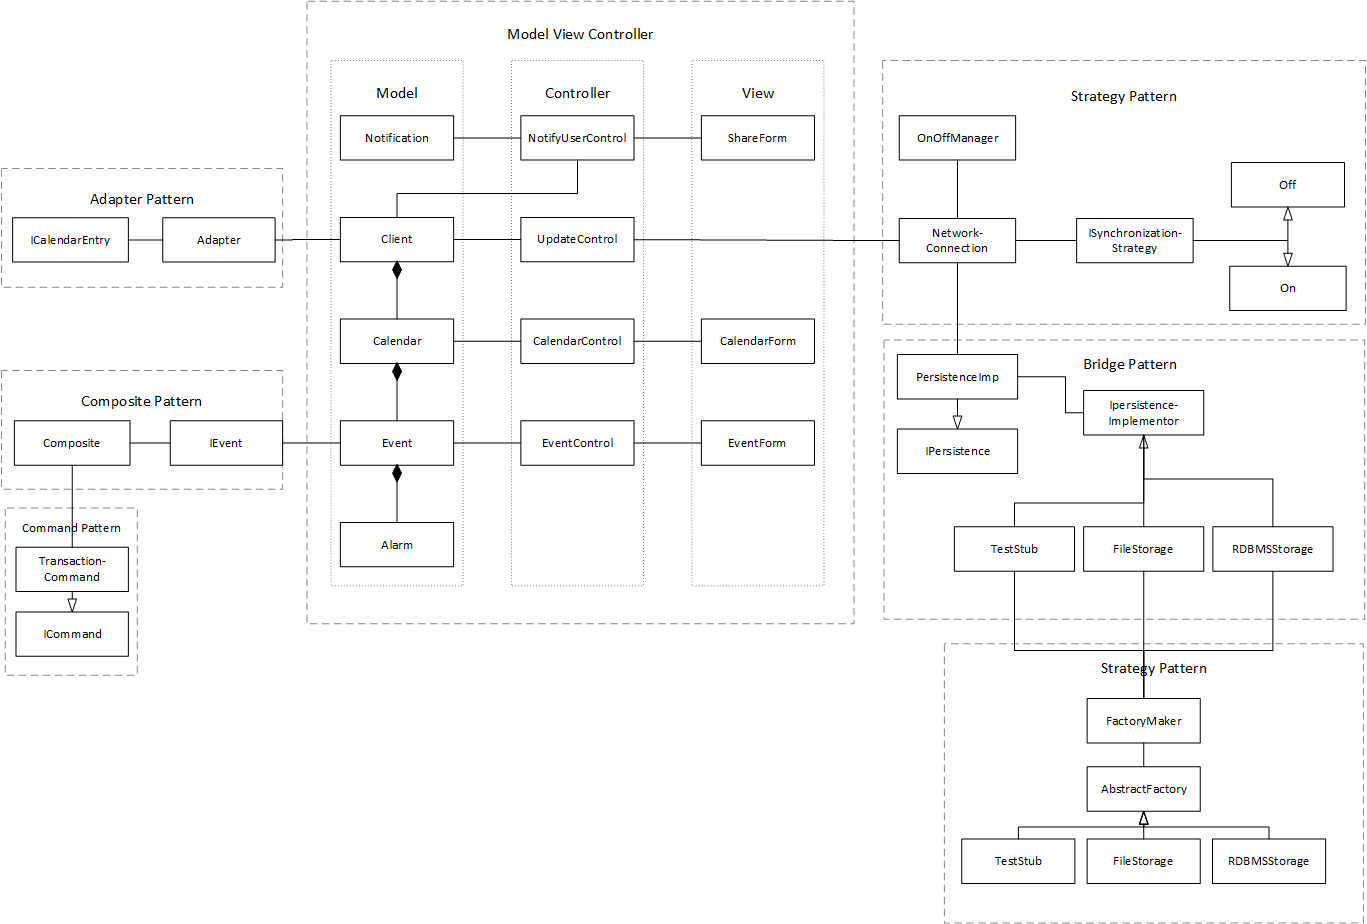
\includegraphics[width=210mm]{class.png}
\caption{UML Class diagram \label{overflow}}
\end{sidewaysfigure}


\clearpage
\section*{Subsystem decomposition}
The subsystem CalendarManagement is the system where most of the program is placed. This system is responsible for all the local events happening in the system. This means that it would handle creation of the calendar, events and provide the necessary GUI for the local program. 

This subsystem has two connections outside the subsystem itself. The first one goes to "ShareInterface" that has all the necessary functions that the CalendarManagement system could ask for when it is about to share a calendar or an event. The other outgoing connection is to the SyncInterface. This is an interface that holds all the needed method calls to synchronize the calendar. Behind the two interfaces we have the subsystems ShareManagement and SyncManagement. 
\newline
\newline
The Share Management has to do with sending the information to the right people and using the right systems. The reason why we made this an interface is that it has been a commonly thing to share through facebook and other social media platforms. Therefore it would be nice to easily have the opportunity to extend the share option so that it would support e.g. Facebook. 
\newline
\newline
The subsystem SyncManagement is where we keep our calendars up to date, where we got the information, of whom the calendar belongs to, and which users that are invited to see it. The syncManagement keep the client calendars synchronized and handles the updates between the local calendar and the online ones. This is also behind an interface so that we can easily exchange it. That would turn to our advantage so the maintenance and upgrades of the system could be done easy. You simply exchange the subsystem part with a new one. E.g. if we wanted to update our synchronization part with a newer version of a data base program, the syncManagement is exchanged, but the rest could stay intact. 
\newline
\begin{figure}[ht!]
\centering
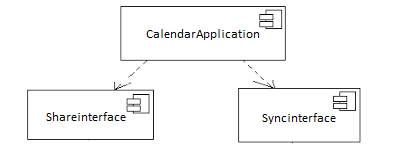
\includegraphics[width=90mm]{diagram.png}
\end{figure}


\newpage
\section*{Hardware/software mapping}

Our Calendar system is run by two devices. The user program run on the user computer, and the synchronized parts will be on the server together with our share system. The two devices will have a connection to each other, we have not yet decided which kind of connection it would be.

\begin{figure}[ht!]
\centering
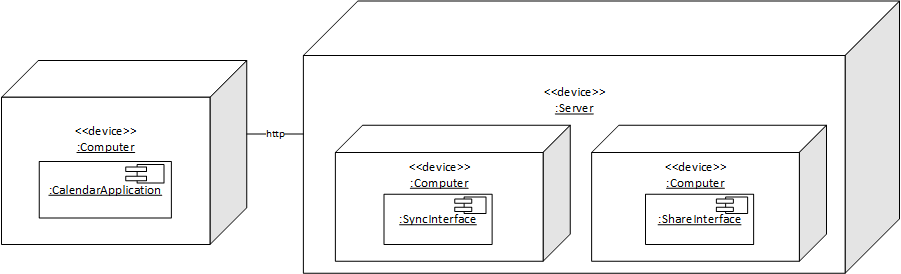
\includegraphics[width=160mm]{UMLDeployment.png}
\caption{UML Deployment diagram \label{overflow}}
\end{figure}

Now that we have mapped our program to the hardware that is used to run our system we dicoverred that some informations had to be handled between the computer and the server. Therefore we have made up a Component Diagram with the subsystems. If we study the ‘ManagingSubSystem’ the ‘SyncSubSystem’ and the ‘ShareSubSystem’, we find that they all have instances of the same classes. This information kept in these instances has to be transfered from the computer to the server via a network connection. Here commes the ‘ControlSubSystem’ in play, this is our subsystem that handles the information and connection between the ‘SyncSubSystem’ and the ‘ManagingSubSystem. The last subsystem ‘CommunicationSubSystem’ will handle the connection to the ‘ShareSubSystem’

\begin{figure}[ht!]
\centering
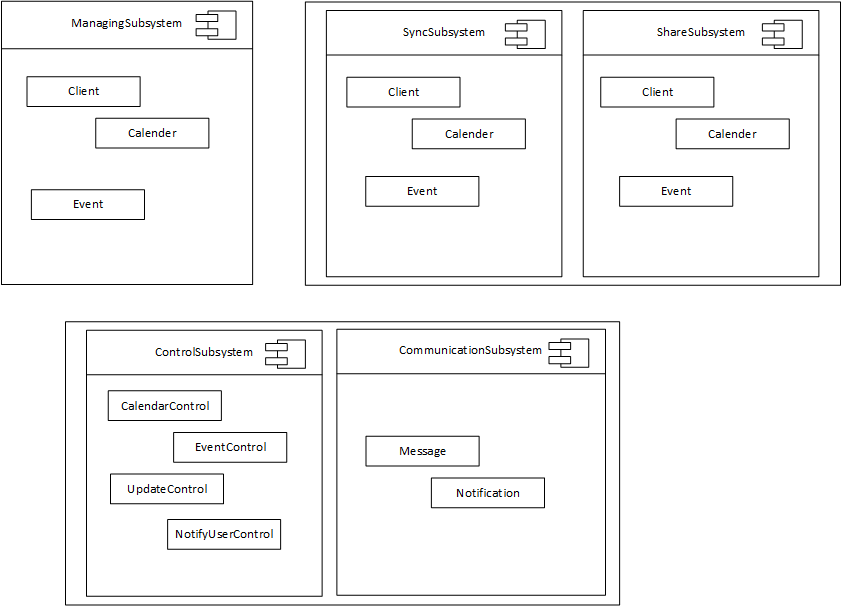
\includegraphics[width=160mm]{UMLComponent.png}
\caption{UML Component diagram \label{overflow}}
\end{figure}


\clearpage
\section*{Persistent data management}
\subsection{Persistent data}
\begin{figure}[ht!]
\centering
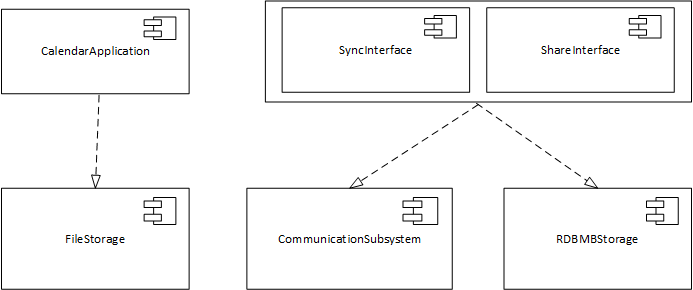
\includegraphics[width=160mm]{UMLComponentData.png}
\caption{Subsystem decomposition with data stores (UML Component diagram) \label{overflow}}
\end{figure}

\textbf{LocalStoreSubsystem} is responsible for storing the data from the calendar on the computer. This functionality is used before the system is synchronized. When synchronized, the data is stored in DBStorageSubsystem, and the data in LocalStoreSubsystem is deleted. 

\textbf{DBStorageSubsystem} is responsible for storing all data from ManageSubsystem in a database for the server. 


\subsection*{Selecting strategy}
\begin{itemize}
	\item In the LocalStoreSubsystem the data is stored as flat files in plain text. 
	\item Data in DBStorageSubsystem is stored in af Relational Database. 
\end{itemize}

\clearpage
\section*{Access control and security}

In fact that our program have multiple users it good to clarify what functions that are available for the different users in the three states a Calendar can be. The three states that our calendar can be in is.

\begin{itemize}
	\item The Global: This Calendar is visible to all users, that subscribe, but it can only be edited by the Client that made the Calendar.
	\item The Local: This Calendar is the one that the Client have shared with his friends, family og coworkers. Both the Client and the subscribing clients have the opportunity see and edit events. The Client that created the Calendar, off course as the only one has the possibility to delete the Calendar.
	\item The Account: The Calendar that can only be seen and edited by the Client that it was created by. 
\end{itemize}

With those informations in the back of our head we made an Access Matrix to get a better view of our Objects Actors functions or method calls available at the different states of a Calendar. 

\begin{tabular}{|p{2.9cm}|p{3.6cm}|p{3.6cm}|p{3.6cm}|}
\hline
\textbf{Object Actors}
&
\textbf{Global}
&
\textbf{Local}
&
\textbf{Account} \\
\hline
\textbf{Client}
& 
\begin{itemize}
\item getCalender() 
\item setCalender() 
\item getEvent()
\item setEvent()
\item unsubscribe()
\item getUser()
\item save()
\item delete()
\end{itemize} 
& 
\begin{itemize}
\item getCalender() 
\item setCalender() 
\item getEvent() 
\item setEvent()
\item unsubscribe()
\item getUser()
\item save()
\item delete()
\end{itemize} 
&
\begin{itemize}
\item getCalender() 
\item setCalender() 
\item getEvent() 
\item setEvent()
\item unsubscribe()
\item getUser()
\item save()
\item delete()
\end{itemize} 
 \\ \hline
\textbf{Server}
& 
\begin{itemize}
\item update()
\end{itemize} 
& 
\begin{itemize}
\item update()
\end{itemize} 
&
\begin{itemize}
\item update()
\end{itemize} 
 \\ \hline
\textbf{Subscribing Client}
& 
\begin{itemize}
\item getCal()
\item getEvent()
\end{itemize} 
& 
\begin{itemize}
\item getCal()
\item setCal() 
\item getEvent()
\item setEvent()
\item unsubscribe()
\item getusers()
\item save()
\end{itemize}
&
No subscribing clients
 \\ \hline
\end{tabular}

\newpage
\section*{Global software control}

In OOSE section 7.4.4 there is mentioned three types of control flow paradigms. 

\begin{itemize}
	\item Procedure-driven control: Operations will wait for an input from actor whenever data is needed. 
	\item Event-driven control: The control flow is determined by events.
	\item Threads: This is a concurrent version of procedure-driven control.
\end{itemize}

 Below is a UML sequence diagram for creating and sharing a calendar:

\begin{figure}[ht!]
\centering
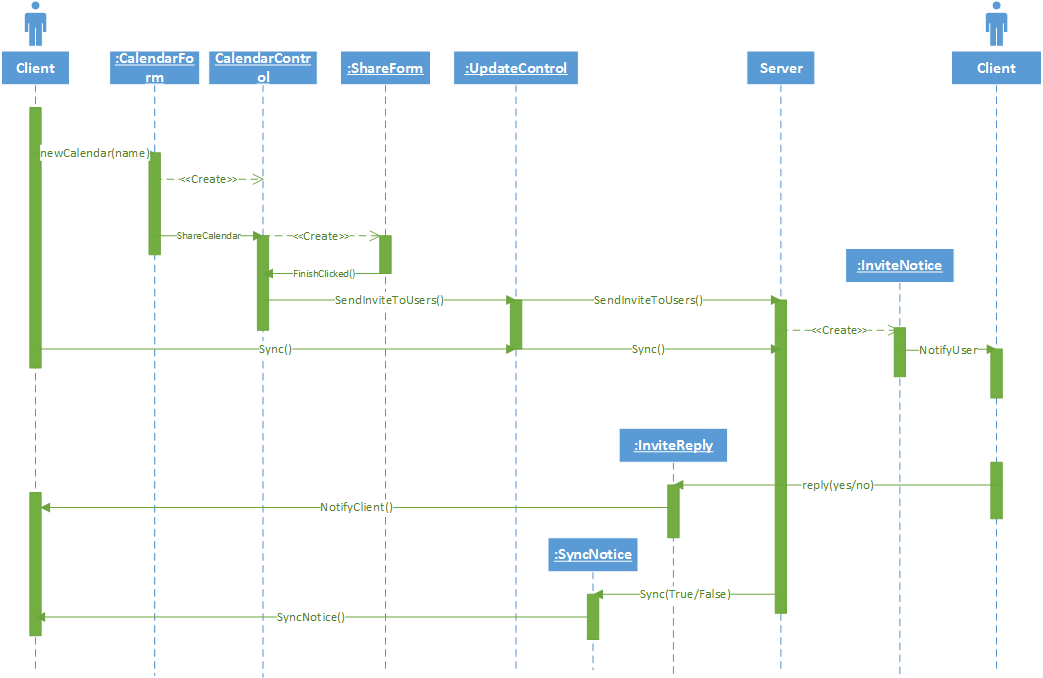
\includegraphics[width=160mm]{UMLSequenceCalendar.png}
\caption{UML Sequence diagram for creating and sharing a calendar \label{overflow}}
\end{figure}

 Events determines the control flow of the system. The design of the control flow will be event-driven. 

\newpage
\section*{Boundary conditions}
\textbf{Start program}
To start the program you must be on a computer with the program on it. Then you just have to run the file. If you want the program to have the full functionality at synchronize the calendar, you must have a network connection. 
\newline
\newline
\textbf{Shutdown program}
To shut down the program you must be in the program, and be able to click on the lock down button. 
We have also clarified some boundary use cases that we have put in our use case diagram, to handle some different boundary exceptions. 


\begin{figure}[ht!]
\centering
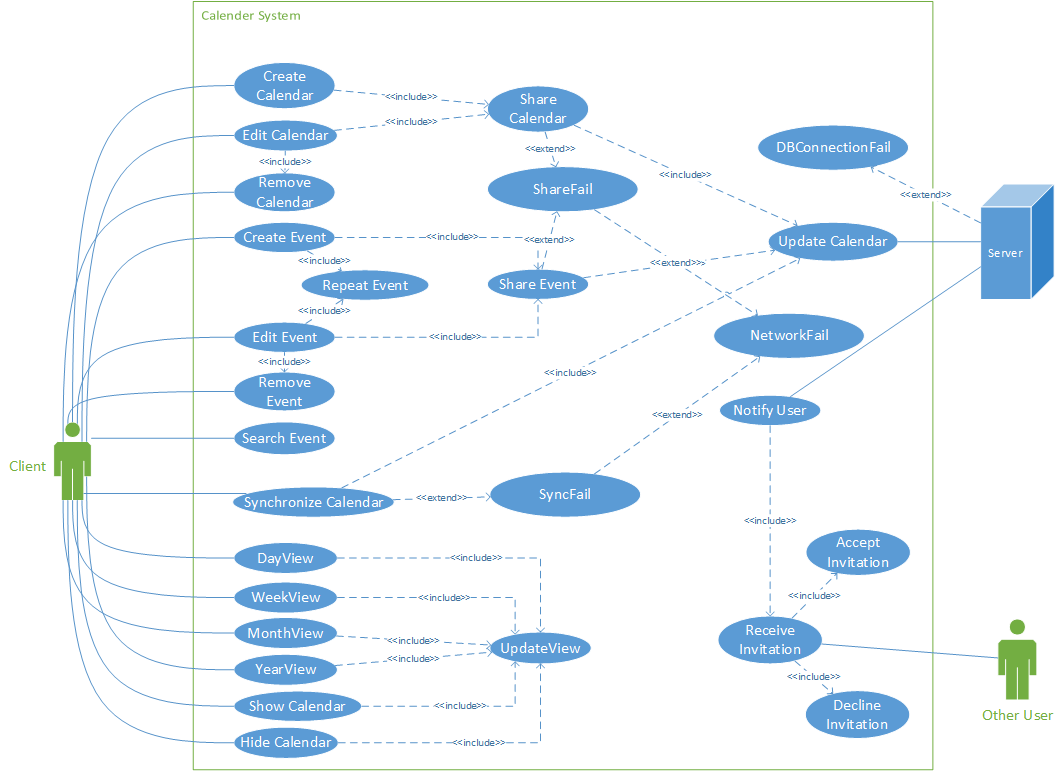
\includegraphics[width=160mm]{usecase.png}
\caption{Updated UML Use Case diagram with  boundary conditions \label{overflow}}
\end{figure}


\newpage
\chapter*{Subsystem services}

\begin{itemize}
	\item ConnectionManager allows a subsystem to register with the CommunicationSubsystem and ControlSubsystem and communicate.
	\item CalculatorRequester allows a subsystem to request a list of available calendars selected trips.
	\item CalendarProvider allows a subsystem to provide a list of calendar that are available for the client and the subscribing clients. 
\end{itemize}

\begin{figure}[ht!]
\centering
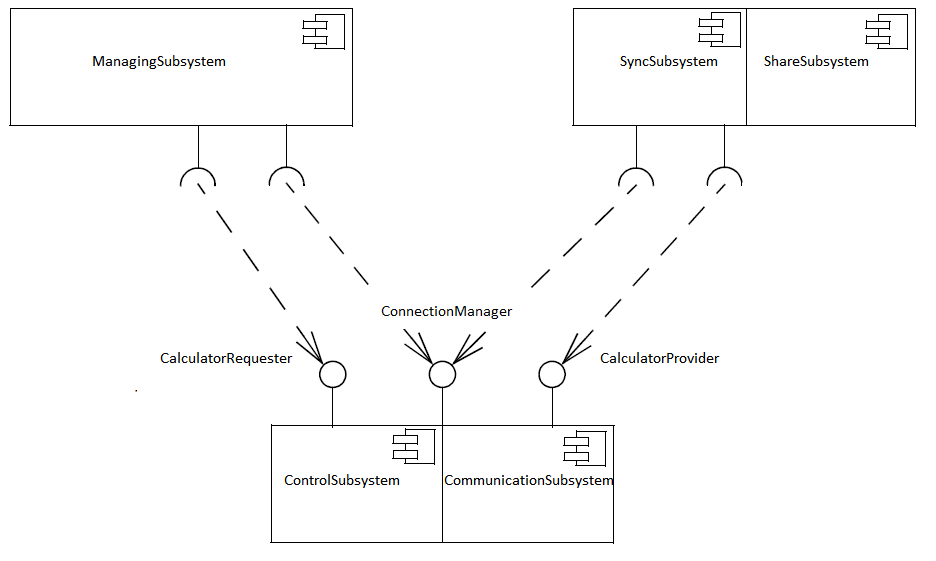
\includegraphics[width=160mm]{UMLComponentService.png}
\caption{Subsystem decomposition with services (UML Component diagram) \label{overflow}}
\end{figure}

\end{document}